\documentclass[a4paper, 10pt, ]{article}

\usepackage[slovak]{babel}





\usepackage[utf8]{inputenc}
\usepackage[T1]{fontenc}

\usepackage[left=4cm,
			right=4cm,
            % left=2.5cm,
			% right=5.5cm,
			top=2.1cm,
			bottom=2.6cm,
			footskip=7.5mm,
			% twoside,
			marginparwidth=3.0cm,
			%showframe,
			]{geometry}

\usepackage{graphicx}
\usepackage[dvipsnames]{xcolor}
% https://en.wikibooks.org/wiki/LaTeX/Colors


% ------------------------------

\usepackage{lmodern}

\usepackage[tt={oldstyle=false,proportional=true,monowidth}]{cfr-lm}

% ------------------------------

\usepackage{amsmath}
\usepackage{amssymb}
\usepackage{amsthm}

\usepackage{booktabs}
\usepackage{multirow}
\usepackage{array}
\usepackage{dcolumn}


\usepackage[singlelinecheck=true]{subfig}


% ------------------------------


\def\naT{\mathsf{T}}

\hyphenpenalty=6000
\tolerance=1000




% ------------------------------


\makeatletter

	\def\@seccntformat#1{\protect\makebox[0pt][r]{\csname the#1\endcsname\hspace{4mm}}}

	\def\cleardoublepage{\clearpage\if@twoside \ifodd\c@page\else
	\hbox{}
	\vspace*{\fill}
	\begin{center}
	\phantom{}
	\end{center}
	\vspace{\fill}
	\thispagestyle{empty}
	\newpage
	\if@twocolumn\hbox{}\newpage\fi\fi\fi}

	\newcommand\figcaption{\def\@captype{figure}\caption}
	\newcommand\tabcaption{\def\@captype{table}\caption}

\makeatother


% ------------------------------




\usepackage{fancyhdr}
\fancypagestyle{plain}{%
\fancyhf{} % clear all header and footer fields
\fancyfoot[C]{\sffamily {\bfseries \thepage}\ | {\scriptsize\oznacenieCasti}}
\renewcommand{\headrulewidth}{0pt}
\renewcommand{\footrulewidth}{0pt}}
\pagestyle{plain}


% ------------------------------


\usepackage{titlesec}
\titleformat{\paragraph}[hang]{\sffamily  \bfseries}{}{0pt}{}
\titlespacing*{\paragraph}{0mm}{3mm}{1mm}
\titlespacing*{\subparagraph}{0mm}{3mm}{1mm}

\titleformat*{\section}{\sffamily\Large\bfseries}
\titleformat*{\subsection}{\sffamily\large\bfseries}
\titleformat*{\subsubsection}{\sffamily\normalsize\bfseries}






% ------------------------------

\PassOptionsToPackage{hyphens}{url}
\usepackage[pdfauthor={},
			pdftitle={},
			pdfsubject={},
			pdfkeywords={},
			% hidelinks,
			colorlinks=false,
			breaklinks,
			]{hyperref}


% ------------------------------


\graphicspath{%
{../fig_standalone/}%
{../../PY/fig/}%
{../../PY/jupynotex/fig/}%
{../../ML/fig/}%
{./fig/}%
}



% ------------------------------

\usepackage{enumitem}

\usepackage{lettrine}

% ------------------------------


\usepackage{microtype}


% ------------------------------

\usepackage[titles]{tocloft}

\setlength{\cftsecindent}{-12mm}
\setlength{\cftsecnumwidth}{12mm}
\renewcommand{\cftsecpresnum}{\hfill}
\renewcommand{\cftsecaftersnum}{\hspace{4mm}}

\setlength{\cftsubsecindent}{-12mm}
\setlength{\cftsubsecnumwidth}{16mm} % 12 + 4
\renewcommand{\cftsubsecpresnum}{\hfill}
\renewcommand{\cftsubsecaftersnum}{\hspace{8mm}} % 4 + 4 mm

\setlength{\cftsubsubsecindent}{-12mm}
\setlength{\cftsubsubsecnumwidth}{20mm} % 12 + 4 + 4
\renewcommand{\cftsubsubsecpresnum}{\hfill}
\renewcommand{\cftsubsubsecaftersnum}{\hspace{12mm}} % 4 + 4 + 4 mm

\renewcommand{\cftsecpagefont}{\lstyle \bfseries}
\renewcommand{\cftsubsecpagefont}{\lstyle}
\renewcommand{\cftsubsubsecpagefont}{\lstyle}



\setlength{\cftparaindent}{-16mm}
\setlength{\cftparanumwidth}{28mm} % 16 + 4 + 4 + 4
\renewcommand{\cftparapresnum}{\hfill}
\renewcommand{\cftparaaftersnum}{\hspace{16mm}} % 4 + 4 + 4 + 4 mm








% ------------------------------

\usepackage{listings}



\renewcommand{\lstlistingname}{Výpis kódu}
\renewcommand{\lstlistlistingname}{Výpisy kódu}




%New colors defined below
\definecolor{codegreen}{rgb}{0,0.6,0}
\definecolor{codegray}{rgb}{0.5,0.5,0.5}
\definecolor{codepurple}{rgb}{0.58,0,0.82}
\definecolor{backcolour}{rgb}{0.95,0.95,0.95}

%Code listing style named "mystyle"
\lstdefinestyle{mystyle}{
  backgroundcolor=\color{backcolour},
  commentstyle=\fontfamily{lmtt}\fontsize{8.5pt}{8.75pt}\selectfont\color{codegreen},
  keywordstyle=\fontfamily{lmtt}\fontsize{8.5pt}{8.75pt}\selectfont\bfseries\color{Blue},
  stringstyle=\fontfamily{lmtt}\fontsize{8.5pt}{8.75pt}\selectfont\color{codepurple},
  basicstyle=\fontfamily{lmtt}\fontsize{8.5pt}{8.75pt}\selectfont,
  breakatwhitespace=false,
  breaklines=true,
  captionpos=t,
  keepspaces=true,
  numbers=left,
  numbersep=4mm,
  numberstyle=\fontfamily{lmtt}\fontsize{8.5pt}{8.75pt}\selectfont\color{lightgray},
  showspaces=false,
  showstringspaces=false,
  showtabs=false,
  tabsize=2,
  % xleftmargin=10pt,
  framesep=10pt,
  language=Python,
  escapechar=|,
}


\lstset{
    inputencoding=utf8,
    extendedchars=true,
    literate=%
    {á}{{\'a}}1
    {č}{{\v{c}}}1
    {ď}{{\v{d}}}1
    {é}{{\'e}}1
    {ě}{{\v{e}}}1
    {í}{{\'i}}1
    {ň}{{\v{n}}}1
    {ó}{{\'o}}1
    {ř}{{\v{r}}}1
    {š}{{\v{s}}}1
    {ť}{{\v{t}}}1
    {ú}{{\'u}}1
    {ů}{{\r{u}}}1
    {ý}{{\'y}}1
    {ž}{{\v{z}}}1
    {Á}{{\'A}}1
    {Č}{{\v{C}}}1
    {Ď}{{\v{D}}}1
    {É}{{\'E}}1
    {Ě}{{\v{E}}}1
    {Í}{{\'I}}1
    {Ň}{{\v{N}}}1
    {Ó}{{\'O}}1
    {Ř}{{\v{R}}}1
    {Š}{{\v{S}}}1
    {Ť}{{\v{T}}}1
    {Ú}{{\'U}}1
    {Ů}{{\r{U}}}1
    {Ý}{{\'Y}}1
    {Ž}{{\v{Z}}}1
    {ô}{{\^{o}}}1
}


% ------------------------------


\usepackage{caption}

\DeclareCaptionFormat{odsadene}{\protect\makebox[0pt][r]{#1#2\hspace{4mm}}#3\par}
\DeclareCaptionLabelSeparator{lendvojbodka}{:}
% \DeclareCaptionFont{lightgray}{\color{lightgray}}
\DeclareCaptionFont{lightgray}{\fontfamily{lmtt}\fontsize{8.5pt}{8.75pt}\selectfont\color{lightgray}}

\captionsetup[lstlisting]{format=odsadene, labelsep=lendvojbodka, justification=raggedright, singlelinecheck=false, labelfont={sf, lightgray},}


% ------------------------------





% ------------------------------

\usepackage[backend=biber,
            style=numeric,
            sorting=none,
            ]{biblatex}
\DeclareSourcemap{
    \maps[datatype=bibtex]{
        \map{
        \step[fieldset=note, null]
        }
        \map{
        \step[fieldset=file, null]
        }        
        % \map{
        % \step[fieldset=url, null]        
        % }
        \map{
        \step[fieldset=eprint, null]
        }
    }
}


\addbibresource{E:/_CurrentContent/01_work_repo/bibLaTeXDB/bibLaTeXDB.bib} % nonpublic data





\def\oznacenieCasti{MRS02 - ZS2022}



\usepackage{pdflscape}
\usepackage{longtable}



\begin{document}


\lstset{%
style=mystyle,
rangebeginprefix=\#\#\#\ cellB\ ,%
rangebeginsuffix=\ \#\#\#,%
rangeendprefix=\#\#\#\ cellE\ ,%
rangeendsuffix=\ \#\#\#,%
includerangemarker=false,
}




\fontsize{12pt}{22pt}\selectfont

\centerline{\textsf{Modelovanie a riadenie systémov} \hfill \textsf{\oznacenieCasti}}

\fontsize{18pt}{22pt}\selectfont





\begin{flushleft}
	\textbf{\textsf{Dynamický systém, diferenciálne rovnice (analytické a numerické riešenie)}}
\end{flushleft}





\normalsize

\bigskip

{\hypersetup{hidelinks}

\tableofcontents

}

\bigskip

\vspace{18pt}



% \noindent
% \lettrine[lines=3, nindent=0pt]{C}{ieľom} tohto textu je najmä vytvoriť akýsi úvodný zoznam pojmov, s ktorými potrebuje čitateľ pracovať pri štúdiu v oblasti kybernetiky, robotiky, teórie riadenia a tak podobne. Vo všeobecnosti ide o~značne široké pojmy avšak v~tomto texte je možné vidieť ako sa s nimi pracuje z hľadiska technickej kybernetiky, z~hľadiska (technickej) teórie systémov, z~hľadiska automatizácie a~z~hľadiska riadiacich systémov.






\section{O dynamickom systéme}



\subsection{Kyvadlo}
\label{castKyvadlo}



\lettrine[lines=3, nindent=0pt]{U}{važujme} kyvadlo, ktorého kmity sú tlmené viskóznym trením s~koeficientom $\beta$ [kg~m$^2$~s$^{-1}$]. Kyvadlo je na Obr.~\ref{Kyvadlo}, kde hmotný bod s~hmotnosťou $m$ [kg] pripevnený na ramene so zanedbateľnou hmotnosťou a~dĺžkou $l$ [m] kmitá, $o$~označuje os otáčania kolmú na rovinu, v~ktorej kyvadlo kmitá, uhol medzi zvislicou a~ramenom kyvadla je označený $\varphi$ [rad] a~gravitačné zrýchlenie $g$~[m~s$^{-2}$].



\begin{center}

	\makebox[\textwidth][c]{%
	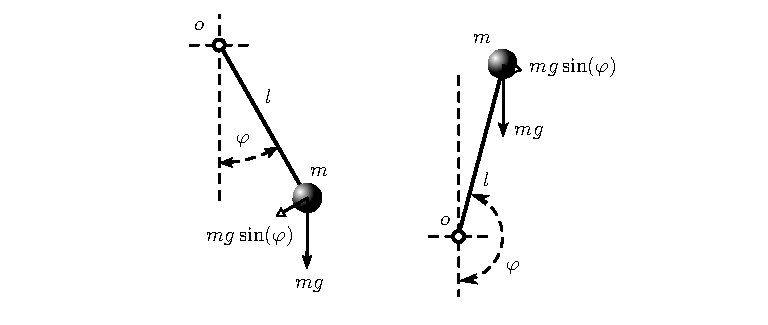
\includegraphics{Obr_Kyvadlo.pdf}
	}
	\vspace{-9mm}

	\figcaption{Kyvadlo}
	\label{Kyvadlo}

	\vspace{-3mm}
\end{center}


Pohybová rovnica opisujúca dynamiku rotačného pohybu kyvadla je v tvare
\begin{subequations} \label{PohRovKyvadla}
\begin{align}
		&ml^2 \ddot{\varphi} + \beta \dot{\varphi} + mgl\sin{\varphi} = u \label{PohRovKyvadlab} \\
		&ml^2 \ddot{\varphi} = -\beta \dot{\varphi} - mgl\sin{\varphi} + u
\end{align}
\end{subequations}
kde $u(t)$ [kg~m$^2$~s$^{-2}$] je externý moment sily pôsobiaci na rameno kyvadla, $\dot{\varphi}(t)$ [rad~s$^{-1}$] je uhlová rýchlosť a~$\ddot{\varphi}(t)$~[rad~s$^{-2}$] je uhlové zrýchlenie ramena kyvadla. Číselné hodnoty parametrov kyvadla sú uvedené v tabuľke~\ref{Parametre kyvadla}.



\begin{table}[b]
	\centering
	\catcode`\-=12


\caption{Parametre kyvadla}
\label{Parametre kyvadla}
\begin{tabular}{     c    c   c       }
\toprule
Parameter   & Hodnota    & Jednotky              \\
\midrule
$m$       & $1$   & kg             \\
$l$    &  $1$  & m \\
$g$   & $9,81$  & m s$^{-2}$ \\
$\beta$  &  $2 \cdot 0,5 \cdot \sqrt{g/l}$ &  kg~m$^2$~s$^{-1}$ \\
\bottomrule
\end{tabular}
\end{table}







\subsection{Modelovanie dynamického systému vo všeobecnosti}


Rovnica \eqref{PohRovKyvadla} je modelom uvažovaného dynamického systému. Model je matematická reprezentácia v tomto prípade fyzikálneho systému. Model umožňuje uvažovať o~systéme a~predpovedať ako sa bude systém správať. Uvedený model opisuje vstupno-výstupné správanie sa dynamického systému, kde vstupom je externý moment sily $u$ a~výstupom je uhol $\varphi$, avšak budeme pracovať aj opisom systému v~\uv{stavovom priestore}.

Stav systému je súbor premenných (súbor veličín), ktoré sumarizujú minulosť systému pre potreby predpovede budúcnosti systému. Pre fyzikálny systém je stav zložený z premenných potrebných pre výpočet zmeny hmotnosti, hybnosti a energie. Kľúčovou otázkou pri vytváraní modelu je ako presne má byť táto zmena popísaná.

Stavové premenné tvoria vektor $x \in  \mathbb{R}^n$, ktorý sa nazýva \emph{stavový vektor}. Vstupy, pomocou ktorých je systém riadený, tvoria vektor vstupov $u \in \mathbb{R}^p$ a~merateľné výstupy systému tvoria vektor výstupov $y \in \mathbb{R}^q$. V~tomto prípade máme $p = q = 1$. Dynamický systém  potom možno reprezentovať rovnicami v~tvare
\begin{subequations} \label{GeneralLTIsyst}
\begin{align}
	\dot{x} &= f(x,u) \\
	y &= h(x,u)
\end{align}
\end{subequations}
kde $f: \mathbb{R}^n \times \mathbb{R}^p \rightarrow \mathbb{R}^n$ a~$h: \mathbb{R}^n \times \mathbb{R}^p \rightarrow \mathbb{R}^q$ sú hladké funkcie. Model v takomto tvare nazývame \emph{model v~stavovom priestore}.





Rozmer stavového vektora sa nazýva \emph{rád systému}. Systém \eqref{GeneralLTIsyst} sa nazýva \emph{časovo-invariantný} pretože funkcie $f$ a $h$ nie sú priamo závislé na čase $t$. Pri časovo-variantných systémoch sú. Model pozostáva z~dvoch funkcií: funkcia $f$ určuje rýchlosť zmeny stavového vektora ako funkciu stavu $x$~a~vstupu $u$, a~funkcia $h$~určuje merateľné výstupy ako funkciu stavu $x$ a vstupu $u$.

Systém sa nazýva lineárny ak sú funkcie $f$~a~$h$~lineárne vzhľadom na $x$~a~$u$. Lineárny model v stavovom priestore má tvar
\begin{subequations} \label{LinearLTIsyst}
\begin{align}
	\dot{x} &= Ax + Bu \\
	y &= Cx + Du
\end{align}
\end{subequations}
kde $A$, $B$, $C$ a $D$ sú konštantné matice. Takýto systém sa nazýva lineárny a časovo-invariantný, v skratke LTI z anglického linear and time-invariant. Matica $A$ sa nazýva dynamická matica, matica $B$ sa nazýva vstupná matica, matica $C$ sa nazýva výstupná matica a matica $D$ sa nazýva priamy člen. Drvivá väčšina systémov nemá priamy člen, čo znamená, že vstup nemá priamy vplyv na výstup.











Iná forma lineárnych diferenciálnych rovníc, ktorá je zovšeobecnením avšak linearizovanej dynamickej rovnice kyvadla (o linearizácii neskôr), má tvar
\begin{align} \label{vseobDifRov}
	\frac{\text{d}^n y}{\text{d}t^n} + a_{n-1} \frac{\text{d}^{(n-1)} y}{\text{d}t^{(n-1)}} + \cdots + a_0 y = b_0 u
\end{align}
kde $t$ je nezávisle premenná (čas), $y(t)$ je závisle premenná (výstup) a $u(t)$ je vstup. Zápis $\frac{\text{d}^n y}{\text{d}t^n}$ značí $n$-tú deriváciu $y$ podľa času $t$ (namiesto $n$ bodiek). Hovoríme, že rovnica \eqref{vseobDifRov} je diferenciálna rovnica $n$-tého rádu, ktorá modeluje dynamiku systému $n$-tého rádu. Tento model môže byť konvertovaný na model v stavovom priestore napríklad definovaním stavového vektora v~tvare
\begin{align}
	x
	=
	\begin{bmatrix}
		x_1 \\ x_2 \\ \vdots \\ x_n
	\end{bmatrix}
	=
	\begin{bmatrix}
		y \\ \frac{\text{d}y}{\text{d}t} \\ \vdots \\ \frac{\text{d}^{(n-1)} y}{\text{d}t^{(n-1)}}
	\end{bmatrix}
\end{align}
potom model v stavovom priestore možno zapísať v~tvare
\begin{subequations}
\begin{align}
	\frac{\text{d}}{\text{d}t}
	\begin{bmatrix}
		x_1 \\ x_2 \\ \vdots \\ x_n
	\end{bmatrix}
	&=
	\begin{bmatrix}
		x_{n-1} \\ x_{n-2} \\ \vdots \\ -a_{n-1} x_n - \cdots - a_0 x_1
	\end{bmatrix}
	+
	\begin{bmatrix}
		0 \\ 0 \\ \vdots \\ b_0 u
	\end{bmatrix}
	\\
	y &= x_1
\end{align}
\end{subequations}
čo po vhodnej definícii matíc $A$, $B$, $C$ a $D$ má tvar \eqref{LinearLTIsyst}.

Ešte všeobecnejší systém získame ak výstup bude lineárnou kombináciou všetkých stavových veličín (predpokladáme, že výstup nezávisí priamo od vstupu), teda
\begin{align}
	y = c_1 x_1 + c_2 x_2 + \cdots + c_n x_n
\end{align}
Potom model v stavovom priestore je
\begin{subequations}
\begin{align}
%\begin{split}
	\dot{x}
	&
	=
	%&
	\begin{bmatrix}
  	0      & 1      & 0      & \cdots & 0      & 0      \\
   	0      & 0      & 1      & \ddots & 0      & 0      \\
    \vdots & \vdots & \ddots & \ddots & \ddots & \vdots \\
    0      & 0      & 0      & \ddots & 1      & 0      \\
    0      & 0      & 0      & \cdots & 0      & 1      \\
   	-a_0   & -a_1   & -a_2   & \cdots &-a_{n-2}&-a_{n-1}
	\end{bmatrix}
	\begin{bmatrix}
		x_1 \\ x_2 \\ \vdots \\ x_{n-2} \\x_{n-1}  \\ x_n
	\end{bmatrix} +
	%&
	\begin{bmatrix}
		0 \\ 0 \\ \vdots \\ 0 \\0  \\ b_0
	\end{bmatrix}
	u
%\end{split}
\\
y &= \begin{bmatrix}
		c_1& c_2 & \hdots & c_{n-2} & c_{n-1}  &c_n
	\end{bmatrix}
	x
\end{align}
\end{subequations}




\subsection{Kyvadlo ako dynamický systém}

Vráťme sa späť k nelineárnym dynamický systémom.


Máme rovnicu opisujúcu dynamiku rotačného pohybu kyvadla. Rovnica je v tvare
\begin{equation}
    ml^2 \ddot{\varphi}(t) + \beta \dot{\varphi}(t) + mgl\sin{\varphi(t)} = u(t)
\end{equation}
Túto rovnicu (rovnicu \eqref{PohRovKyvadlab}) možno prepísať aj na tvar
\begin{align}
	\ddot{\varphi} = - \frac{\beta}{ml^2} \dot{\varphi} - \frac{g}{l} \sin(\varphi) + \frac{1}{ml^2}u
\end{align}
čo je v tomto prípade úprava len kozmetická, ale relatívne užitočná, ako sa ukáže.


\paragraph{Analytické a numerické riešenie}

Samozrejme, ide o diferenciálnu rovnicu. Presnejšie o obyčajnú diferenciálnu rovnicu 2. rádu, ktorá je nehomogénna (vyskytuje sa v nej „externý signál“ (vstup)). Cieľom je nájsť riešenie tejto rovnice pre dané začiatočné podmienky a pre prípadné dané vstupy (vstupné signály).

Analytické riešenie diferenciálnej rovnice je v podstate nejaká funkcia času (a~prípadne iných veličín). Numerické riešenie je postupnosť hodnôt, číselných hodnôt, ktoré pri daných predpokladoch vyhovujú diferenciálnej rovnici. Je to postupnosť hodnôt - vektor hodnôt, ku ktorému prislúcha časový vektor určujúci časovú postupnosť hodnôt numerického riešenia. Tu sme vynechali pár miliónov detailov, ale snáď sa dá vytušiť, čo sa tu myslí pod numerickým riešením.




\subsubsection{Rovnica vyššieho rádu ako sústava rovníc 1. rádu}
\label{RVRASR1R}

Každú diferenciálnu rovnicu vyššieho rádu je možné zapísať ako sústavu rovníc prvého rádu. Napríklad sústavu dvoch rovníc prvého rádu je možné vo všeobecnosti zapísať v tvare
\begin{equation} \label{naznak01}
   \begin{bmatrix} \dot x_1(t) \\ \dot x_2(t) \end{bmatrix} = F \left( t, \begin{bmatrix} x_1(t) \\ x_2(t) \end{bmatrix}, \ldots \right)
\end{equation}


V takejto novej sústave rovníc, vo všeobecnosti, vznikli nové veličiny (signály), ktoré sa vo všeobecnosti môžu líšiť od pôvodných veličín (signálov) v pôvodnej rovnici vyššieho rádu.


Nové veličiny vystupujúce v sústave rovníc sa v teórii systémov súhrnne označujú ako stav systému (stavové veličiny systému). Ak poznáme aktuálny stav systému potom spravidla vieme určiť predchádzajúce aj budúce stavy (vo všeobecnosti).

Napr. v rovnici kyvadla vystupujú veličiny (signály) $\ddot \varphi(t)$, $\dot \varphi(t)$ a~$\varphi(t)$. Je zrejmé (možno nie nad slnko jasné), že ako stav systému je možné zvoliť veličiny $\varphi(t)$ a $\dot \varphi(t)$, teda polohu a~uhlovú rýchlosť kyvadla. Ak poznáme tieto, poznáme celú históriu a~budúcnosť pohybu kyvadla.

Môže existovať viac možností voľby stavových veličín. Pri lineárnych systémoch je možností nekonečne veľa (nekonečne veľa stavových priestorov). Z praktického hľadiska však majú význam len niektoré voľby - napr. pri pohybových systémoch, akým je kyvadlo, sú to prirodzene polohy, rýchlosť, zrýchlenie, trh atď., v~závislosti od rádu systému.



Jednou z možností ako previesť rovnicu vyššieho rádu na sústavu rovníc prvého rádu je nasledovný postup. V tomto prípade je zhodou okolností výsledkom aj prakticky využiteľný stavový priestor (stavové veličiny $\varphi(t)$ a $\dot \varphi(t)$). Nech
\begin{equation}
    x_1(t) = \varphi(t)
\end{equation}
potom
\begin{equation}
    \dot x_1(t) = \dot \varphi(t)
\end{equation}
Ďalej nech
\begin{equation}
    \dot x_1(t) = \dot \varphi(t) = x_2(t)
\end{equation}
a to znamená, že
\begin{equation}
    \dot x_2(t) = \ddot \varphi(t)
\end{equation}
Tým sme získali veličiny $x_1(t) = \varphi(t)$ a $x_2(t) = \dot \varphi(t)$. Je možné zostaviť stavový vektor $x = \begin{bmatrix} x_1(t) & x_2(t) \end{bmatrix}^\mathsf T$ a teda $\dot x = \begin{bmatrix} \dot x_1(t) & \dot x_2(t) \end{bmatrix}^\mathsf T$.





\bigskip

\noindent
Ako sme naznačili v súvislosti s \eqref{naznak01}, cieľom je vlastne konkretizovať funkciu $F$ v~rovnici
\begin{equation}
    \dot x = F(t, x, \ldots)
\end{equation}
čo je kompaktný zápis sústavy
\begin{align}
    \dot x_1(t) &= F_1 \left(t, x_1(t), x_2(t), \ldots \right) \\
    \dot x_2(t) &= F_2 \left(t, x_1(t), x_2(t), \ldots \right)
\end{align}

Prvú rovnicu v tomto prípade máme:
\begin{equation}
    \dot x_1(t) = x_2(t)
\end{equation}
Druhá rovnica vyplynie z postrehu, že pôvodnú rovnicu druhého rádu možno zapísať v tvare
\begin{align}
    \begin{split}
    \ddot \varphi(t) &= -\frac{\beta}{ml^2}\dot\varphi(t) - \frac{g}{l} \sin\left( \varphi(t) \right) + \frac{1}{ml^2} u(t) \\
                     &= -\frac{\beta}{ml^2} x_2(t) - \frac{g}{l} \sin\left( x_1(t) \right) + \frac{1}{ml^2} u(t)
    \end{split}
\end{align}
kde sú využité novo zavedené stavové veličiny $x_1(t)$ a $x_2(t)$. Je zrejmé, že druhá rovnica sústavy je
\begin{equation}
    \dot x_2(t) = -\frac{\beta}{ml^2} x_2(t) - \frac{g}{l} \sin\left( x_1(t) \right) + \frac{1}{ml^2} u(t)
\end{equation}
a teda rovnice kyvadla v stavovom priestore sú
\begin{align} \label{rovniceKyvSSpredpis}
    \begin{bmatrix} \dot x_1(t) \\ \dot x_2(t)  \end{bmatrix} = \begin{bmatrix} x_2(t) \\ -\frac{\beta}{ml^2} x_2(t) - \frac{g}{l} \sin\left( x_1(t) \right)  \end{bmatrix} + \begin{bmatrix} 0 \\ \frac{1}{ml^2} \end{bmatrix} u(t)
\end{align}
čím je funkcia $F$ jasne stanovená.

\paragraph{Zhrňme}

Stavom kyvadla sú dve veličiny: uhol natočenia ramena kyvadla $\varphi$ a~uhlová rýchlosť ramena kyvadla $\dot\varphi$. Stavový vektor má preto dva prvky $x^{\mathsf{T}} = \begin{bmatrix} x_1 & x_2	\end{bmatrix}$, kde $x_1 = \varphi$ a~$x_2 = \dot\varphi$. Model kyvadla v stavovom priestore je v tvare
\begin{subequations}
	\begin{align}
		\begin{bmatrix}
			\dot{x}_1 \\ \dot{x}_2
		\end{bmatrix}
		&=
		\begin{bmatrix}
			x_2 \\ - \frac{\beta}{ml^2} x_2 - \frac{g}{l} \sin(x_1)
		\end{bmatrix}
		+
		\begin{bmatrix}
			0 \\ \frac{1}{ml^2}
		\end{bmatrix}
		u \\
		\varphi &= x_1
	\end{align}
\end{subequations}
Toto je nelineárny časovo-invariantný systém druhého rádu.



















\section{O analytickom riešení diferenciálnych rovníc}



\subsection{Príklad s vybíjaním kondenzátora}

Pripomeňme, že diferenciálna rovnica opisujúca vybíjanie kondenzátora je v tvare
\begin{equation} \label{diffRbeta}
    \frac{\text{d}Q(t)}{\text{d}t} = - \frac{1}{RC} Q(t) \qquad Q(0) = Q_0
\end{equation}
(podrobnosti boli vedené v inom (predchádzajucom) dokumente).

Len pre zovšeobecnenie, zmeňme označenia v tejto rovnice (v snahe o univezálnejší zápis):
\begin{equation} \label{prerobDR}
    \dot y(t) = -a y(t)  \qquad y(0) = y_0
\end{equation}
kde $y(t)$ je hľadaná časová funkcia, $a>0$ a $y_0$ je tzv. začiatočná hodnota (funkcie $y(t)$). Ide o obyčajnú lineárnu diferenciálnu rovnicu (prípadne hovoríme len lineárna diferenciálna rovnica, skratkou LDR). Tiež môžme písať
\begin{equation} \label{prerobDR2}
    \dot y(t) + a y(t) = 0
\end{equation}
a teda vidíme, že rovnica (alebo teda dynamický systém, ktorý opisuje) je homogénna, teda nemá „vstup“, nemá „pravú stranu“. Preto celkové riešenie rovnice hľadáme ako lineárnu kombináciu fundamentálnych riešení.

Pre hľadanie fundamentálnych riešení sa využíva postup s využitím tzv. \emph{charakteristickej rovnice}.

% \paragraph{Nie len ku charakteristickej rovnici:}
%
% \begin{itemize}[leftmargin=0pt, labelsep=3mm, itemsep=0pt]
%     \scriptsize
%     \item \url{https://cs.wikipedia.org/wiki/Charakteristick%C3%A1_rovnice}
% 	\item \url{https://www.math.sk/skripta2/node88.html}
%     \item \url{http://thales.doa.fmph.uniba.sk/sleziak/texty/gyurki/diferaky/dif.pdf}
%     \item \url{https://math.libretexts.org/Courses/Monroe_Community_College/MTH_225_Differential_Equations/9%3A_Linear_Higher_Order_Differential_Equations/9.2%3A_Higher_Order_Constant_Coefficient_Homogeneous_Equations}
% 	\item atď, atď\ldots
% \end{itemize}

Zostavme charakteristickú rovnicu prislúchajúcu k diferenciálnej rovnici \eqref{prerobDR}. Charakteristická rovnica v tomto prípade je:
\begin{equation}
    s + a = 0
\end{equation}
Pre úplnosť, charakteristický polynóm je teda v tomto prípade:
\begin{equation}
    s + a
\end{equation}
Riešením charakteristickej rovnice (v ktorej premenná $s$ teraz vlastne predstavuje len akúsi neznámu), alebo koreňom charakteristického polynómu je:
\begin{equation}
    s_1 = -a
\end{equation}
Keďže je len jedno riešenie charakteristickej rovnice, tak je len jedno fundamentálne riešenie. Totiž, vo všeobecnosti možno rozlišovať niekoľko prípadov, pre ktoré platí:
\begin{enumerate}[leftmargin=0pt, labelsep=4mm, itemsep=0pt]
    \item Ak má charakteristická rovnica $n$ navzájom rôznych riešení $s_i$ pre $i = 1, \ldots, n$, potom zodpovedajúce fundamentálne riešenia (módy) sú: $e^{s_1 t}$, $e^{s_2 t}$, \ldots, $e^{s_n t}$.
    \item Ak sa medzi $n$ koreňmi charakteristického polynómu vyskytne $k$-násobný koreň, vytvoríme $k$ lineárne závislých riešení: $e^{s_i t}$, $t e^{s_i t}$, \ldots, $t^{k-1} e^{s_i t}$
    \item V prípade výskytu dvojice komplexne združených koreňov charakteristického polynómu, $s_{1,2} = \alpha \pm j \beta$, kde $j$ je imaginárna jednotka, využijeme na určenie fundamentálnych riešení Eulerov vzťah
    \begin{equation}
        e^{\left(\alpha \pm j \beta\right)t} = e^{\alpha t} \left( \cos\beta t \pm j \sin \beta t\right)
    \end{equation}
    Preto potom možno písať príslušné fundamentálne riešenie v tvare
    \begin{equation}
        c_1 e^{\left(\alpha + j \beta\right)t} + c_2 e^{\left(\alpha - j \beta\right)t} = e^{\alpha t} \left( c^\prime \cos\beta t + c^{\prime\prime} \sin \beta t\right)
    \end{equation}
    kde sú imaginárne časti nulové.
\end{enumerate}



 V tomto prípade teda fundamentálne riešenie je:
 \begin{equation}
      y_{f1}(t) = e^{s_1 t} = e^{(-a) t}
 \end{equation}

Celkové riešenie je lineárna kombinácia fundamentálnych riešení, v tomto prípade jednoducho:
\begin{equation}
     y(t)  = c_1 e^{(-a) t}
\end{equation}
kde $c_1$ je konštanta (reálne číslo). Táto konštanta má vo všeobecnosti neznámu hodnotu. Avšak, ak sú dané začiatočné podmienky pre LDR, potom je túto konštantu (alebo viac konštánt ak by bolo viac fundamentálnych riešení) možné určiť na základe začiatočných podmienok. Pre začiatok, teda čas 0, platí
\begin{equation}
     y(0)  = c_1 e^{(-a) 0} = c_1
\end{equation}
A samotná hodnota $y(0)$ je známa, kežďe máme začiatočnú podmienku $y(0) = y_0$. Takže
\begin{equation}
     c_1 = y_0
\end{equation}
To znamená, že riešenie diferenciálnej rovnice je:
\begin{equation}
     y(t)  = y_0 e^{(-a) t}
\end{equation}











\subsection{Príklad 2}


Majme diferenciálnu rovnicu
\begin{align}
    \ddot y(t) + 3\dot y(t) + 2 y(t) = 0 \qquad y(0)=3, \dot y(0) = -2
\end{align}
Nájdime funkciu $y(t)$, ktorá je riešením diferenciálnej rovnice.

Určme charakteristickú rovnicu:
\begin{align}
    s^2 +3s + 2 = 0
\end{align}
Jej korene sú
\begin{align}
    s_{1, 2} = \frac{-3 \pm \sqrt{3^2 + 4\cdot1\cdot2}}{2\cdot1} = \frac{-3 \pm \sqrt{1}}{2}
\end{align}
a teda
\begin{align}
    s_1 = -2 \qquad s_2 = -1
\end{align}

Lineárna kombinácia fundamentálnych riešení potom je
\begin{align} \label{lkombfunp2}
    y(t) = c_1 e^{-2t} + c_2 e^{-t}
\end{align}
Konštanty $c_1$ a $c_2$ nájdeme využitím začiatočných podmienok. Začiatočné podmienky určujú hodnoty pre $y(0)$ a pre $\dot y(0)$. Preto nás zaujímajú aj $y(t)$ a $\dot y(t)$. Všeobecný predpis pre $y(t)$ už máme - \eqref{lkombfunp2}. Práve z neho je možné získať aj predpis pre $\dot y(t)$, keďže ide o $\frac{\text{d}}{\text{d}t}y(t)$, a ten je
\begin{subequations}
    \begin{align}
        \dot y(t) &= c_1 e^{-2t} (-2) + c_2 e^{-t} (-1) \\
        \dot y(t) &= -2 c_1 e^{-2t} - c_2 e^{-t}
    \end{align}
\end{subequations}

Potom, na základe podmienok zhody musí platiť
\begin{subequations}
    \begin{align}
        y(0) &= c_1 + c_2 = 3 \\
        \dot y(0) &= -2 c_1  - c_2  = -2
    \end{align}
\end{subequations}
Takže $c_2 = 3-c_1$, a teda
\begin{subequations}
    \begin{align}
         -2 c_1  - 3 + c_1 &= -2 \\
         -c_1 &= 1 \\
         c_1 &= -1
    \end{align}
\end{subequations}
a
\begin{align}
     c_2 = 4
\end{align}

Našli sme funkciu $y(t)$, ktorá je riešením diferenciálnej rovnice:
\begin{align}
     y(t) = - e^{-2t} + 4 e^{-t}
\end{align}




\subsection{Príklad pre širší rozhľad}
\label{Príklad pre širší rozhľad}


Majme diferenciálnu rovnicu:
\begin{equation} \label{Zadaná rovnica}
	\dddot{y} + 5,4 \ddot{y} + 9,7 \dot{y} + 5,592 y = 2 e^{-1,2t}
\end{equation}

\noindent
Pre tento dynamický systém zvoľme nenulové začiatočné podmienky nasledovne:
\begin{equation*}
		y(0) = 1 \qquad \dot{y}(0)  = 1 \qquad 	\ddot{y}(0) = 1
\end{equation*}



\bigskip


\noindent
Rovnica \eqref{Zadaná rovnica} je nehomogénna lineárna diferenciálna rovnica s konštantnými koeficientami tretieho rádu ($n_r = 3$). Jej Charakteristická rovnica je
\begin{equation}
	s^3 + 5,4 s^2 + 9,7 s + 5,592 = 0
\end{equation}
Riešeniami Charakteristickej rovnice sú
\begin{equation} \label{Korene CHR}
		s_1 = -2,1 + 0,5i \qquad
		s_2 = -2,1 - 0,5i \qquad
		s_3 = -1,2
\end{equation}
Fundamentálne riešenia (módy) rovnice \eqref{Zadaná rovnica} zodpovedajúce jednotlivým riešeniam Charakteristickej rovnice sú
\begin{subequations}
	\begin{align}
		y_1(t) &= e^{(-2,1 + 0,5i)t} = e^{-2,1t} \big({ \cos(0,5t) + i\sin(0.5t) }\big) \\
		y_2(t) &= e^{(-2,1 - 0,5i)t} = e^{-2,1t} \big({ \cos(0,5t) - i\sin(0.5t) }\big) \\
		y_3(t) &= e^{-1.2t}
	\end{align}
\end{subequations}



Totiž, vo všeobecnosti možno rozlišovať niekoľko prípadov, pre ktoré platí:
\begin{enumerate}[leftmargin=0pt, labelsep=4mm, itemsep=0pt]
    \item Ak má charakteristická rovnica $n$ navzájom rôznych riešení $s_i$ pre $i = 1, \ldots, n$, potom zodpovedajúce fundamentálne riešenia (módy) sú: $e^{s_1 t}$, $e^{s_2 t}$, \ldots, $e^{s_n t}$.
    \item Ak sa medzi $n$ koreňmi charakteristického polynómu vyskytne $k$-násobný koreň, vytvoríme $k$ lineárne závislých riešení: $e^{s_i t}$, $t e^{s_i t}$, \ldots, $t^{k-1} e^{s_i t}$
    \item V prípade výskytu dvojice komplexne združených koreňov charakteristického polynómu, $s_{1,2} = \alpha \pm j \beta$, kde $j$ je imaginárna jednotka, využijeme na určenie fundamentálnych riešení Eulerov vzťah
    \begin{equation}
        e^{\left(\alpha \pm j \beta\right)t} = e^{\alpha t} \left( \cos\beta t \pm j \sin \beta t\right)
    \end{equation}
    Preto potom možno písať príslušné fundamentálne riešenie v tvare
    \begin{equation}
        c_1 e^{\left(\alpha + j \beta\right)t} + c_2 e^{\left(\alpha - j \beta\right)t} = e^{\alpha t} \left( c^\prime \cos\beta t + c^{\prime\prime} \sin \beta t\right)
    \end{equation}
    kde sú imaginárne časti nulové.
\end{enumerate}


Výsledné reálne všeobecné riešenie homogénnej časti má tvar
\begin{equation} \label{Výsledné reálne všeobecné riešenie homogénnej}
	y_{h_{vs}}(t) = c_1 e^{-2,1t} \cos(0,5t) + c_2 e^{-2,1t} \sin(0,5t) + c_3 e^{-1.2t}
\end{equation}
kde $c_1$, $c_2$ a $c_3$ sú reálne konštanty.







Pravá strana $q(t)$ diferenciálnej rovnice \eqref{Zadaná rovnica} má vo všeobecnosti tvar $q(t) = e^{\alpha t} P_n(t)$, pričom platí
\begin{subequations}
	\begin{align}
		P_n(t) &= 2 \\
		\alpha &= -1,2
	\end{align}
\end{subequations}
Pre tento špeciálny tvar pravej strany má partikulárne riešenie $\psi(t)$ tvar $\psi(t) = t^k e^{\alpha t} Q_n(t)$, kde $k$ je násobnosť koreňa $\alpha$ a $Q_n(t)$ je všeobecný polynóm rovnakého stupňa ako $P_n(t)$. V tomto prípade
\begin{subequations}
	\begin{align}
		k &= 1 \\
		Q_n(t) &= A_0
	\end{align}
\end{subequations}
Partikulárne riešenie $\psi(t)$ určíme použitím metódy neurčitých koeficientov, a teda partikulárne riešenie a jeho derivácie dosadíme do diferenciálnej rovnice.
\begin{subequations} \label{derivacieParRies}
	\begin{align}
		\psi(t) &= A_0 t e^{-1,2 t} \\
		\dot{\psi}(t) &=  A_0 e^{-1,2t} - 1,2 A_0 t e^{-1,2t}\\
		\ddot{\psi}(t) &= -2,4 A_0 e^{-1,2t} + 1,44 A_0 t e^{-1,2t} \\
		\dddot{\psi}(t) &= 4,32 A_0 e^{-1,2t} - 1,728 A_0 t e^{-1,2t}
	\end{align}
\end{subequations}
Rovnice \eqref{derivacieParRies} dosadíme do diferenciálnej rovnice \eqref{Zadaná rovnica} a upravíme.
\begin{subequations}
\begin{align}
	\begin{split}
		2 e^{-1,2t} &=
		 4,32 A_0 e^{-1,2t} - 1,728 A_0 t e^{-1,2t}  + 5,4 \left( -2,4 A_0 e^{-1,2t} + 1,44 A_0 t e^{-1,2t} \right) \\
		& + 9,7  \left( A_0 e^{-1,2t} - 1,2 A_0 t e^{-1,2t} \right) + 5,592 \left( A_0 t e^{-1,2 t} \right)
	\end{split} \\
	\begin{split}
		2 e^{-1,2t} &=
		 4,32 A_0 e^{-1,2t} - 1,728 A_0 t e^{-1,2t} - 12,96 A_0 e^{-1.2t} + 7,776 A_0 t e^{-1,2t}  \\
		& + 9,7  A_0 e^{-1,2t} - 8,5 A_0 t e^{-1,2t} + 5,592  A_0 t e^{-1,2 t}
	\end{split} \\
	\begin{split} \label{dosadenePartikRies}
		2 e^{-1,2t} &=
		 1,06 A_0 e^{-1,2t} + 3,14 t e^{-1,2 t}
	\end{split}
\end{align}
\end{subequations}
Z \eqref{dosadenePartikRies} vyplýva
\begin{equation}
	2 = 1,06 A_0 \qquad \Rightarrow \qquad A_0 = \frac{2}{1,06} \doteq 1,8868
\end{equation}
a partikulárne riešenie $\psi(t)$ je
\begin{equation} \label{Partikulárne riešenie}
	\psi(t) = 1,8868 t e^{-1,2 t}
\end{equation}






Všeobecné riešenie diferenciálnej rovnice \eqref{Zadaná rovnica} je súčet \eqref{Výsledné reálne všeobecné riešenie homogénnej} s \eqref{Partikulárne riešenie}:
\begin{subequations}
\begin{equation} \label{Všeobecné riešenie}
	y_{vs}(t) = c_1 e^{-2,1t} \cos(0,5t) + c_2 e^{-2,1t} \sin(0,5t) + c_3 e^{-1.2t} + 1,8868 t e^{-1,2 t}
\end{equation}
Konštanty $c_1$, $c_2$ a $c_3$ sú dané konkrétnymi začiatočnými podmienkami, ktoré sa dosadia do príslušných derivácií všeobecného riešenia. V tomto prípade sú potrebné okrem nultej derivácie \eqref{Všeobecné riešenie} aj prvá a druhá derivácia všeobecného riešenia:
\begin{align}
	\begin{split} \label{prvaDer Všeobecné riešenie}
		\dot y_{vs}(t) &= 1,8868e^{-1,2 t}  -2,2642te^{-1,2 t} - 1,2 c_3 e^{-1,2t} - 2,1 c_2 e^{-2,1t} \sin(0,5t) \\&+ 0,5 c_2 e^{-2,1t} \cos(0,5t) - 2,1 c_1 e^{-2,1t} \cos(0,5t) - 0,5 c_1 e^{-2,1t} \sin(0,5t)
	\end{split} \\
	\begin{split} \label{druhaDer Všeobecné riešenie}
		\ddot y_{vs}(t) &= -4,5283 e^{-1.2t} + 2,717 t e^{-1.2t} + 1,44 c_3 e^{-1.2t} + 4,16 c_2 e^{-2.1t} \sin(0.5t) \\&- 2.1 c_2 e^{-2.1t} \cos(0.5t) + 4,16 c_1 e^{-2.1t} \cos(0.5t) + 2.1 c_1 e^{-2.1t} \sin(0.5t)
	\end{split}
\end{align}
\end{subequations}









Dosadením začiatočných podmienok do \eqref{Všeobecné riešenie}, \eqref{prvaDer Všeobecné riešenie} a \eqref{druhaDer Všeobecné riešenie} získame sústavu troch rovníc o troch neznámych, ktorá má v maticovom zápise tvar
\begin{equation}
	\begin{bmatrix}
		   1 &    0 &    1 \\
		-2,1 &  0,5 & -1,2 \\
		4,16 & -2,1 & 1,44
	\end{bmatrix}
	\begin{bmatrix}
		c_1 \\
		c_2 \\
		c_3
	\end{bmatrix}
	=
	\begin{bmatrix}
		1 \\
		1-1,8868 \\
		1+4,5283
	\end{bmatrix}
\end{equation}
a jej riešením je
\begin{subequations}
	\begin{align}
		c_1 &= -5,0979\\
		c_2 &= -8,5498\\
		c_3 &=  6,0979
	\end{align}
\end{subequations}




Riešením diferenciálnej rovnice \eqref{Zadaná rovnica} je
\begin{equation}
	y(t) = -5,0979 e^{-2,1t} \cos(0,5t)  -8,5498 e^{-2,1t} \sin(0,5t) + 6,0979 e^{-1.2t} + 1,8868 t e^{-1,2 t}
\end{equation}
Graficky je riešenie znázornené na Obr. \ref{Grafické znázornenie riešenia získaného analyticky}.


\begin{figure}[!ht]
	\centering

    \makebox[\textwidth][c]{%
	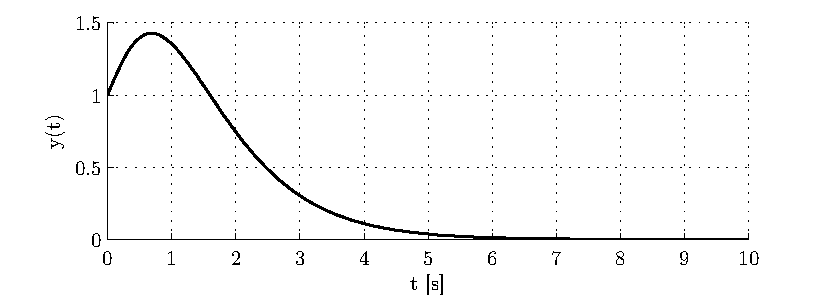
\includegraphics{Obr_GrafRucne.pdf}
    }

	\caption{Grafické znázornenie riešenia získaného analyticky}
	\label{Grafické znázornenie riešenia získaného analyticky}
\end{figure}









\paragraph{Riešenie pomocou Symbolic toolboxu (MATLAB)}



Pre výpočet riešenia pomocou toolboxu Symbolic je potrebné zadať nasledujúce príkazy:
\begin{lstlisting}[language=Matlab,]
yt = dsolve('D3y + 5.4*D2y + 9.7*Dy + 5.592*y = 2*exp(-1.2*t)','y(0)=1','Dy(0)=1','D2y(0)=1')

ezplot(yt,[0 10])
\end{lstlisting}
Odpoveďou je riešenie a vykreslenie jeho priebehu znázornené na Obr. \ref{Grafické znázornenie riešenia získaného Symbolic}.
{\footnotesize
\begin{verbatim}
yt =

100/53*t*exp(-6/5*t)+17129/2809*exp(-6/5*t)-120082/14045*exp(-21/10*t)*sin(1/2*t)
-14320/2809*exp(-21/10*t)*cos(1/2*t)
\end{verbatim}}


\begin{figure}[!ht]
	\centering

    \makebox[\textwidth][c]{%
	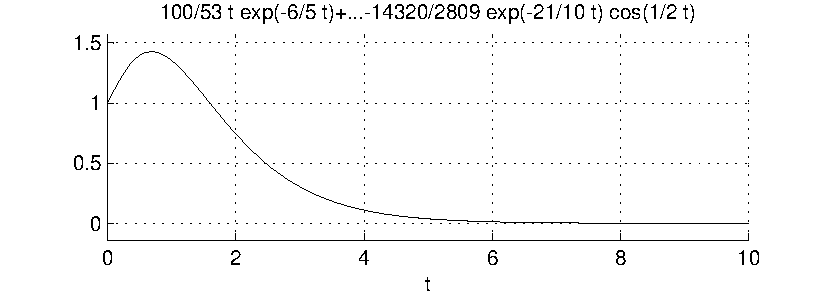
\includegraphics{Obr_Symbolic.pdf}
    }

	\caption{Grafické znázornenie riešenia získaného pomocou toolboxu Symbolic}
	\label{Grafické znázornenie riešenia získaného Symbolic}
\end{figure}













































\section[O numerickom riešení diferenciálnych rovníc (a ODE solver)]{O numerickom riešení diferenciálnych rovníc\\ (a ODE solver)}






\subsection{ODE solver}


Pre hľadanie numerického riešenia využijeme ODE solver. ODE je skratka pre obyčajné diferenciálne rovnice (ordinary differential equation).

Úlohou ODE solvera je nájsť numerické riešenie na základe rovnice (diferenciálnej), ktorú je možné vo všeobecnosti zapísať v tvare
\begin{equation}
    \dot x(t) = f \left( t, x(t), \ldots \right)
\end{equation}
kde $f$ je funkcia, ktorej argumenty sú čas $t$, prirodzene, samotný výstupný (hľadaný, neznámy) signál $x(t)$ a prípadne iné ďalšie parametre či veličiny - napríklad externý vstup. Uvedená rovnica doslova predpisuje aká je časová zmena signálu $x(t)$. Časová zmena signálu, inými slovami časová derivácia (derivácia podľa času) je označená ako $\dot x(t)$.

Ak teda do funkcie $f$ dosadíme hodnoty argumentov (čas, signál $x(t)$, a prípadne iné), získame hodnotu časovej zmeny $\dot x(t)$. Na základe informácie o $\dot x(t)$, ktorá zodpovedá aktuálnemu (dosadenému) signálu $x(t)$, môžeme určiť hodnotu $x(t)$ o~nejaký čas neskôr. Túto novú hodnotu $x(t)$ možno opäť dosadiť do funkcie $f$~a~následne nájsť ďalšiu ešte ďalej v čase - atď. ODE solver využíva práve tento jednoduchý princíp pre postupné hľadanie hodnôt (numerických hodnôt) signálu $x(t)$.

Vo všeobecnosti sa uvedený princíp nazýva numerická integrácia. ODE solver teda numericky integruje. Je množstvo metód pre numerickú integráciu, ktoré sa líšia spôsobom riešenia problémov súvisiacich so samotným procesom numerickej integrácie (voľba (optimalizácia) časového kroku integrácie, zohľadnenie matematických vlastností daného typu diferenciálnych rovníc a iné). ODE solvre sa môžu líšiť aj samotnou implementáciou niektorej z metód numerickej integrácie. Podrobnejší opis ODE solvera je nad rámec tohto textu.












\subsection{Používanie ODE solvera}



ODE solver ako funkcia v programe môže mať napríklad nasledujúce vstupy (argumenty) a výstupy:

\begin{verbatim}
x = odesolver(fcnF, init, timeVect)
\end{verbatim}
kde \verb|x| je, samozrejme, hľadané numerické riešenie. Prvým argumentom je funkcia s názvom \verb|fcnF|, ktorá implementuje sústavu diferenciálnych rovníc v zmysle predchádzajúceho textu. \verb|init| označuje začiatočné hodnoty stavových veličín. \verb|timeVect| označuje časové okamihy (vzorky), v ktorých hľadáme hodnoty numerického riešenia.






\subsubsection{MATLAB}

\noindent
MATLAB obsahuje hneď niekoľko ODE solverov. Tu budeme používať \verb|ode45|.

Vytvorme funkciu, ktorá realizuje sústavu diferenciálnych rovníc \eqref{rovniceKyvSSpredpis}, avšak, uvažujme, že vstupný signál $u(t)$ je nulový. Teda neuvažujme vstupný signál vôbec. Ešte inými slovami, externý moment sily je nulový, $u(t) = 0$ a preto potom možno písať
\begin{align} \label{fajnVektRov0}
	\begin{bmatrix}
		\dot{x}_1 \\ \dot{x}_2
	\end{bmatrix}
	&=
	\begin{bmatrix}
		x_2 \\ - \frac{\beta}{ml^2} x_2 - \frac{g}{l} \sin(x_1)
	\end{bmatrix}
\end{align}
Toto je autonómny nelineárny časovo-invariantný systém druhého rádu. Jeho správanie závisí len od začiatočného stavu na začiatku uvažovaného času.

Funkcia, ktorá realizuje uvedenú sústavu, môže byť nasledovná:


\lstset{style=mystyle}
\begin{lstlisting}[language=Matlab, title=Celý súbor PravaStr.m]
function dotx = PravaStr(t,x)

global m l g beta

dotx1 =  x(2);
dotx2 = - (beta/m*l^2)*x(2)  -  (g/l)*sin(x(1));

dotx = [dotx1; dotx2];

end
\end{lstlisting}


Vytvorme „hlavný skript“, v ktorom všetko potrebné nastavíme a v ktorom budeme volať ODE solver. Ako prvé nech su globálne premenné (v tomto prípade parametre kyvadla):
\begin{lstlisting}[language=Matlab, title=Časť súbora hlSkript.m, name=hlSkript]
global m l g beta

m = 1; %kg
l = 1; %m
g = 9.81; %m/s^2
beta = 2*0.5*sqrt(g/l); %kgm^2/s
\end{lstlisting}
Definujme časový vektor, ktorý určí pre aké časové okamihy ODE solver vráti numerické riešenie:
\begin{lstlisting}[language=Matlab, title=Časť súbora hlSkript.m, name=hlSkript]
timeVect = 0:0.1:5;
\end{lstlisting}
Zavolajme ODE solver, pričom ostáva zvoliť začiatočné podmienky - začiatočný stav kyvadla. Nech začiatočný stav je $x_1(0) = 0.25$ [rad] a~$x_2(0) = 0$ [rad/s].
\begin{lstlisting}[language=Matlab, title=Časť súbora hlSkript.m, name=hlSkript]
[t,x] = ode45(@(t,x) PravaStr(t,x), timeVect, [pi/4; 0]);
\end{lstlisting}
Premenná \verb|x| teraz obsahuje dva stĺpce - prvý stĺpec je prvá stavová veličina a druhý stĺpec je druhá stavová veličina.
Pre nakreslenie vypočítaného riešenia:
\begin{lstlisting}[language=Matlab, title=Časť súbora hlSkript.m, name=hlSkript]
figure(1)
plot(t,x)
\end{lstlisting}
Výsledné numerické riešenie je graficky znázornené na obr.~\ref{cv2obr1}.


\begin{figure}[!ht]
	\centering

	\makebox[\textwidth][c]{%
	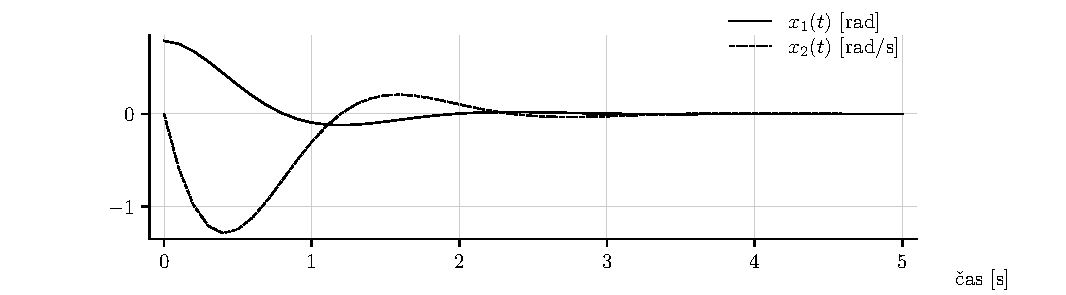
\includegraphics{cv02_fig_1.pdf}
	}

    \vspace{-1mm}

	\caption{Grafické zobrazenie numerického riešenia}
	\label{cv2obr1}
\end{figure}


Na obr.~\ref{cv2obr1} ide však len o akési základné zobrazenie. Zmysluplnejšie by napríklad mohlo byť, ak by sme do grafu nakreslili len priebeh polohy (výchylky) kyvadla samostatne a navyše nie v radiánoch ale v stupňoch -- viď obr.~\ref{cv2obr2}. Pre takýto obrázok možno do hl. skriptu pridať:
\begin{lstlisting}[language=Matlab, title=Časť súbora hlSkript.m, name=hlSkript]
figure(2)
plot(t,x(:,1)*180/pi)
\end{lstlisting}

\begin{figure}[!ht]
	\centering

	\makebox[\textwidth][c]{%
	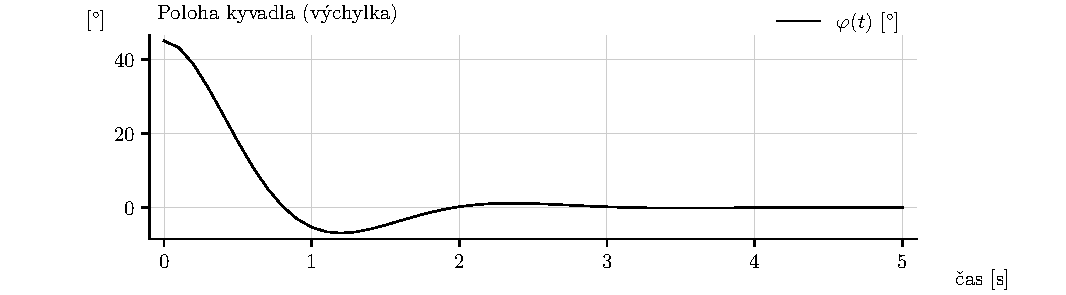
\includegraphics{../fig/cv02_fig_2.pdf}
	}

    \vspace{-1mm}

	\caption{Grafické zobrazenie priebehu polohy kyvadla}
	\label{cv2obr2}
\end{figure}






\subsubsection{Python}

Pre informáciu, nasledovne by vyzeralo hľadanie numerického riešenia v rámci jazyka Python.


Knižnica \href{https://www.scipy.org/}{\color{NavyBlue} SciPy}, presnejšie \href{https://docs.scipy.org/doc/scipy-0.18.1/reference/integrate.html}{\color{NavyBlue} scipy.integrate} obsahuje ODEsolver s názvom \verb|odeint|. Vytvorme skript využívajúci tento ODE solver:


\begin{lstlisting}[language=Python, title=Skript v Python-e]
import numpy as np
from scipy.integrate import odeint
import matplotlib.pyplot as plt

m = 1.0
l = 1.0
g = 9.81
beta = 2 * 0.5 * np.sqrt(g/l)

def fcn_rovniceKyvadla(x, t, u):
    x_1, x_2 = x
    dotx_1 = x_2
    dotx_2 = -(beta/m*l**2) * x_2 - (g/l) * np.sin(x_1) + (1.0/m*l**2) * u
    return [dotx_1, dotx_2]


timeVect = np.arange(0, 5.1, 0.1)

u = 0

x = odeint(fcn_rovniceKyvadla,
           [np.pi/4, 0],   # zaciatocne podmienky
           timeVect,
           args=(u,),
           )

plt.figure(1)
plt.plot(timeVect, x)
plt.xlabel(u'cas [s]')
plt.legend(['$x_1(t)$ [rad]', '$x_2(t)$ [rad/s]'])

plt.figure(2)
plt.plot(timeVect, x[:,0]*180/np.pi)
plt.xlabel(u'cas [s]')
plt.ylabel(u'$x_1(t)$ [stupne]')
\end{lstlisting}


Pozornému čitateľovi iste neuniklo, že uvedený skript v Pythone obsahuje funkciu, ktorá realizuje sústavu diferenciálnych rovníc \eqref{rovniceKyvSSpredpis}, ale v tomto prípade zahŕňa aj vstupnú veličinu $u(t)$. Táto je potom v tomto prípade nastavená na nulovú hodnotu.



\subsection{Ďalšie simulácie s kyvadlom}

\subsubsection{Iné začiatočné podmienky}

Nech začiatočné podmienky (začiatočný stav) sú: $x_1(0) = 0.1$ [rad] a~$x_2(0) = 1$ [rad/s]. Pritom nech vstup $u(t)$ je stále nulový. Výsledok simulácie je na obrázku~\ref{cv2obr3}.
\begin{center}

    \makebox[\textwidth][c]{%
	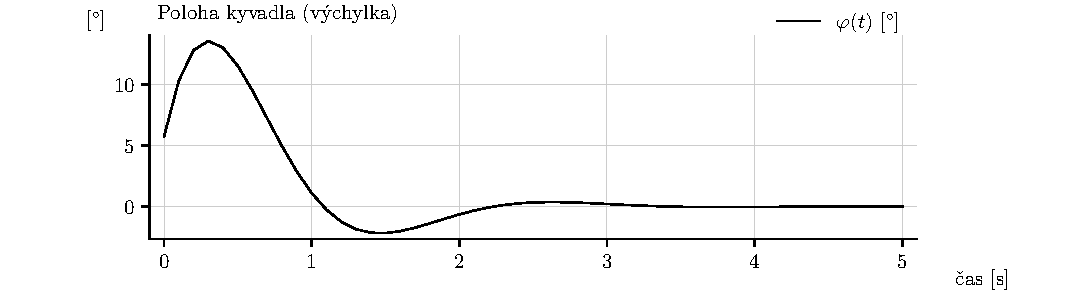
\includegraphics{cv02_fig_3.pdf}
	}

    \vspace{-3mm}

    \figcaption{Grafické zobrazenie priebehu polohy kyvadla}
	\label{cv2obr3}

    % \vspace{-3mm}

\end{center}

\noindent
Ďalšie simulácie s rôznymi začiatočnými podmienkami kyvadla sa ponechávajú na čitateľa.





\subsubsection{Nenulový vstupný signál}

Modifikujme pôvodnú funkciu a skrip v MATLAB-e tak, aby bolo možné simulovať nenulový vstupný signál $u(t)$.

Funkciu, ktorá realizuje sústavu diferenciálnych rovníc \eqref{rovniceKyvSSpredpis} aj so vstupným signálom $u(t)$:
\begin{lstlisting}[language=Matlab, title=Celý súbor PravaStr\_u.m]
function dotx = PravaStr_u(t,x, u)

global m l g beta

dotx1 =  x(2);
dotx2 = - (beta/m*l^2)*x(2) - (g/l)*sin(x(1)) + (1/m*l^2) * u;

dotx = [dotx1; dotx2];

end
\end{lstlisting}

Vytvorme „hlavný skript“, v ktorom všetko potrebné nastavíme a v ktorom budeme volať ODE solver:
\begin{lstlisting}[language=Matlab, title=Súbor hlSkript\_u.m]
global m l g beta

m = 1; %kg
l = 1; %m
g = 9.81; %m/s^2
beta = 2*0.5*sqrt(g/l); %kgm^2/s

u = 3

[t,x] = ode45(@(t,x) PravaStr_u(t,x,u), [0 10], [0; 0]);

figure(3)
plot(t,x(:,1)*180/pi)
\end{lstlisting}

\bigskip

\noindent
Simulujme prípad keď napríklad $u(t) = 3$ [kg m$^2$ s$^{-2}$] (pozn.: pre lepšiu názornosť uvažujme začiatočné podmienky nulové). Výsledok simulácie je na obrázku~\ref{cv2obr4}.
\begin{center}

    \makebox[\textwidth][c]{%
	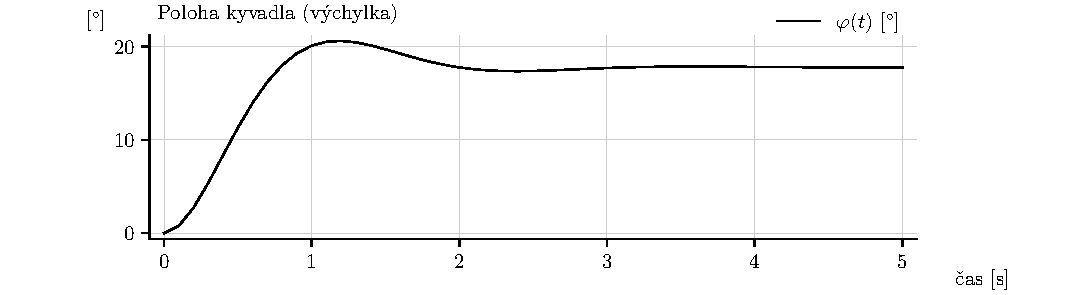
\includegraphics{cv02_fig_4.pdf}
	}

    \vspace{-3mm}

    \figcaption{Grafické zobrazenie priebehu polohy kyvadla}
	\label{cv2obr4}

    % \vspace{-3mm}

\end{center}



Zaujímavý prípad je, keď $u(t) = 9,81$ [kg m$^2$ s$^{-2}$]. Výsledok simulácie je na obrázku~\ref{cv2obr5}.
\begin{center}

    \makebox[\textwidth][c]{%
	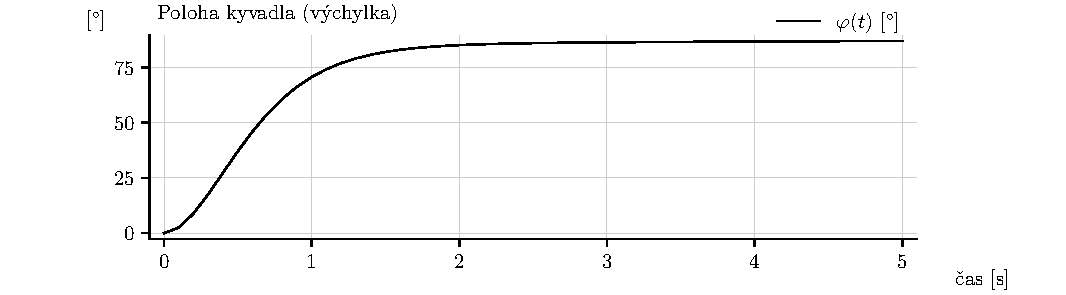
\includegraphics{cv02_fig_5.pdf}
	}

    \vspace{-3mm}

    \figcaption{Grafické zobrazenie priebehu polohy kyvadla}
	\label{cv2obr5}

    % \vspace{-3mm}

\end{center}
Avšak, lepšie sa to ukáže, ak predĺžime časový vektor (čas simulácie) -- viď obrázok~\ref{cv2obr6}. Je zrejmé, že kyvadlo sa približuje k hodnote 90 stupňov.
\begin{center}

    \makebox[\textwidth][c]{%
	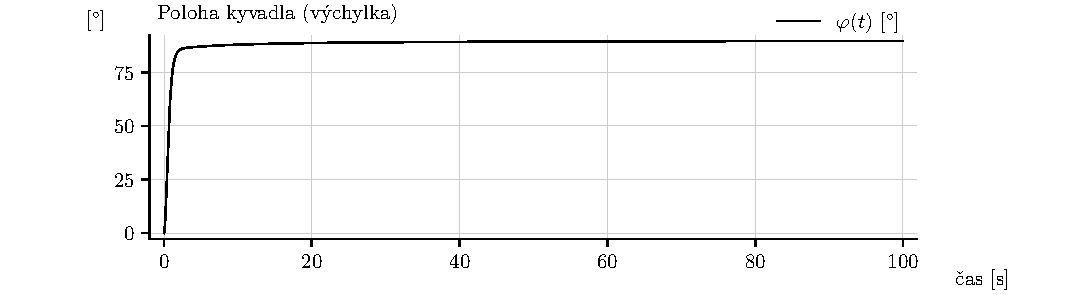
\includegraphics{cv02_fig_6.pdf}
	}

    \vspace{-3mm}

    \figcaption{Grafické zobrazenie priebehu polohy kyvadla}
	\label{cv2obr6}

    % \vspace{-3mm}

\end{center}


Čo sa stane ak $u = 9,82$ [kg m$^2$ s$^{-2}$]? (obr.~\ref{cv2obr7})
\begin{center}

    \makebox[\textwidth][c]{%
	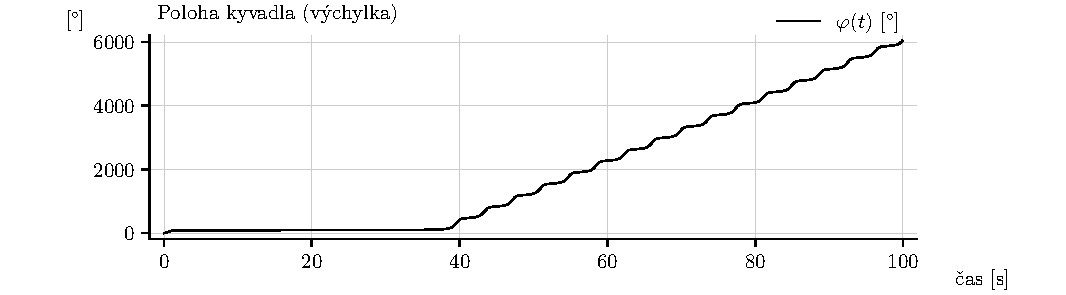
\includegraphics{cv02_fig_7.pdf}
	}

    \vspace{-3mm}

    \figcaption{Grafické zobrazenie priebehu polohy kyvadla}
	\label{cv2obr7}

    % \vspace{-3mm}

\end{center}







\subsection{Numerické riešenie príkladu pre širší rozhľad (z časti~\ref{Príklad pre širší rozhľad})}

Pripomeňme, že máme diferenciálnu rovnicu:
\begin{equation} \label{Zadaná rovnica numpr}
	\dddot{y} + 5,4 \ddot{y} + 9,7 \dot{y} + 5,592 y = 2 e^{-1,2t}
\end{equation}
a pre tento dynamický systém uvažujeme nenulové začiatočné podmienky nasledovne:
\begin{equation*}
		y(0) = 1 \qquad \dot{y}(0)  = 1 \qquad 	\ddot{y}(0) = 1
\end{equation*}




\subsubsection{Simulink}

Simulačná schéma zodpovedajúca diferenciálnej rovnici \eqref{Zadaná rovnica numpr} je na Obr. \ref{Simulačná schéma}. Začiatočné podmienky integrátorov v schéme sú nastavené rovnako ako boli zvolené v zadaní. Simuláciou získaný časový priebeh je na Obr. \ref{Simuláciou získaný časový priebeh}.

\begin{center}

    \makebox[\textwidth][c]{%
	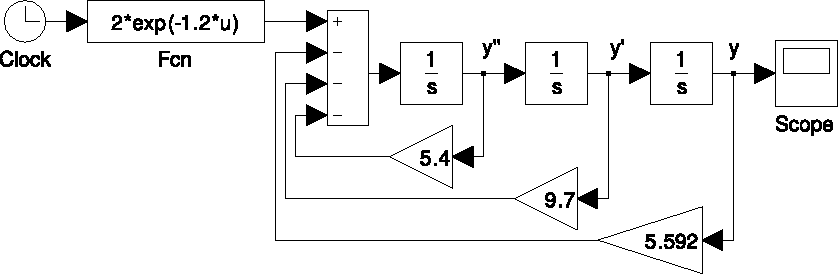
\includegraphics{Obr_SimSchema_FontPokus.pdf}
	}

    \figcaption{Simulačná schéma}
	\label{Simulačná schéma}

\end{center}

\begin{center}

    \makebox[\textwidth][c]{%
	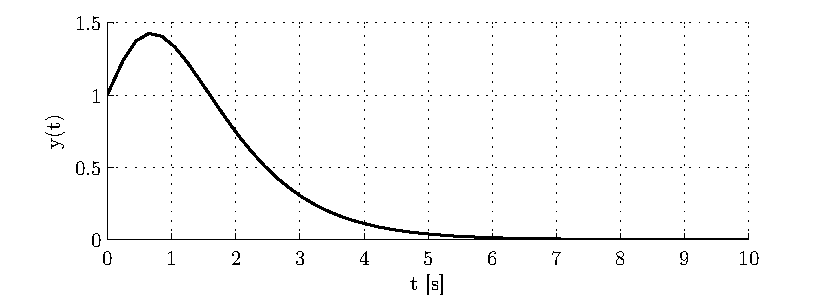
\includegraphics{Obr_Simulink.pdf}
	}

    \figcaption{Simuláciou získaný časový priebeh}
	\label{Simuláciou získaný časový priebeh}

\end{center}




\subsubsection{ODE solver vo všeobecnosti (MATLAB)}

Pre numerický výpočet riešenia pomocou procedúry \verb|ode45| je potrebné previesť diferenciálnu rovnicu \eqref{Zadaná rovnica} na systém diferenciálnych rovníc 1. rádu. V tomto prípade:
\begin{subequations}
	\begin{align}
		\dot x_1 &= x_2 \\
		\dot x_2 &= x_3 \\
		\dot x_3 &= -5,4 x_3 -9,7 x_2 -5,592 x_1 + 2 e^{-1,2 t}
	\end{align}
\end{subequations}
Tento systém sa potom zapíše ako funkcia, ktorú bude procedúra \verb|ode45| používať
\begin{lstlisting}[language=Matlab,]
function dx = fundif(t,x);
dx(1) = x(2);
dx(2) = x(3);
dx(3) = -5.4*x(3) -9.7*x(2) -5.592*x(1) + 2*exp(-1.2*t);
dx = dx(:);
\end{lstlisting}
Samotné použitie procedúry \verb|ode45| sa vykoná nasledovnými príkazmi:
\begin{lstlisting}[language=Matlab,]
[t,y] = ode45('fundif',[0 10],[1; 1; 1]);
plot(t,y(:,1))
\end{lstlisting}
Výsledný priebeh riešenia je na Obr. \ref{Grafické znázornenie riešenia získaného pomocou ode45}.

\begin{center}

    \makebox[\textwidth][c]{%
	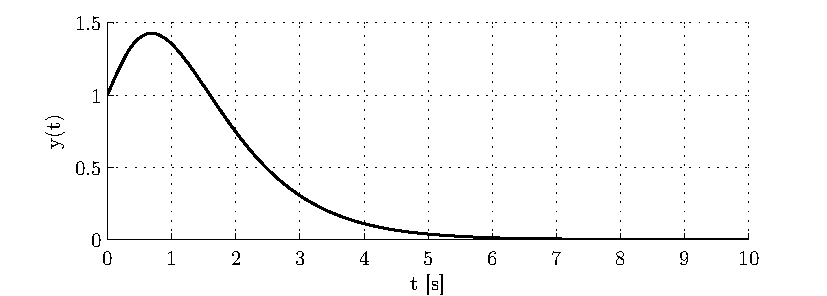
\includegraphics{Obr_ode45.pdf}
	}

    \figcaption{Grafické znázornenie riešenia získaného pomocou ode45}
	\label{Grafické znázornenie riešenia získaného pomocou ode45}

\end{center}






















\section{Cvičenie druhé}

Úlohou je zostaviť numerickú simuláciu, pomocou ktorej je možné simulovať časový priebeh veličín elektromagnetického a mechanického podsystému elektrického motora. Uvažovaným je jednosmerný elektrický motor s cudzím konštantným budením.

Základné informácie o motore: Nominálny výkon \lstyle{39}~[kW], nominálne napätie \lstyle{520}~[V] a~nominálny prúd \lstyle{89}~[A]. Nominálne otáčky motora: \lstyle{1113}~[ot/min] a~nominálny krútiaci moment: \lstyle{337}~[Nm]. Ide teda o relatívne výkonný, veľký motor.

Pre zostavenie matematického modelu motora, s cieľom opísať dynamické deje pri štarte a prevádzke, je potrebné zohľadniť, že ide o prípad s konštantným cudzím budením čo zjednodušuje predovšetkým opis elektromagnetickej časti systému. Zároveň sú v tomto prípade dostupné informácie o tzv. stratách v železe a výsledkom je možnosť uvažovať tzv. napäťovú konštantu motora $C_{u\omega}$ [Vs] a momentovú konštantu motora $C_{uM}$ [Nm/A]. V tomto prípade (bez uvádzania ďalších podrobností) máme
\begin{subequations}
	\begin{align}
		C_{u\omega} &= 3,903\ \text{[Vs]}\\
		C_{uM} &= 3,787\ \text{[Nm/A]}
	\end{align}
\end{subequations}


Elektromagnetický podsystém motora (čo v tomto prípade je v podstate len rotorové vinutie) je možné opísať diferenciálnou rovnicou v tvare
\begin{align} \label{dfsv}
	u(t) = R i(t) + L \frac{\text{d}i(t)}{\text{d}t} + u_i(t)
\end{align}
kde $R$ [$\Omega$] je elektrický odpor vinutia, $L$ [H] je indukčnosť vinutia a $u_i$ je spätné indukované napätie, ktoré je v podstate následkom meniaceho sa magnetického poľa vzhľadom na vinutie. Práve tu sa využije napäťová konštanta motora keď platí $u_i(t) = C_{u\omega} \omega(t)$, kde $\omega(t)$ [rad/s] je uhlová rýchlosť motora. A teda rovnicu \eqref{dfsv} je možné zapísať v tvare
\begin{align} \label{dfsv2}
	u(t) = R i(t) + L \frac{\text{d}i(t)}{\text{d}t} + C_{u\omega} \omega(t)
\end{align}
Číselné hodnoty parametrov v tomto prípade sú: $R = 0,737$~[$\Omega$] a $L = 0,00905$~[H].



Mechanický podsystém motora je možné opísať známou rovnicou
\begin{align} \label{drms}
	M_m(t) = J_m \frac{\text{d}\omega(t)}{\text{d}t}
\end{align}
kde $M_m(t)$ [Nm] je krútiaci moment, ktorý motor produkuje, $J_m$ [kg m${}^2$] je moment zotrvačnosti a $\omega(t)$ [rad/s] je uhlová rýchlosť motora. Moment produkovaný motorom je možné určiť pomocou momentovej konštanty motora vzťahom $M_m(t) = C_{uM} i(t)$. Pozorný čitateľ si tu všimne, že v rovnici \eqref{drms} sa vôbec neuvažuje mechanická záťaž motora (záťažný moment motora), pričom však tento je jednoduché pridať.

Rovnicu \eqref{drms} môžeme v tomto prípade písať aj v tvare
\begin{align} \label{drms2}
	C_{uM} i(t) = J_m \frac{\text{d}\omega(t)}{\text{d}t}
\end{align}
Číselné hodnoty parametrov v tomto prípade sú: $J_m = 0,5$~[kg m${}^2$].



\subsection{Úlohy}

\begin{enumerate}[leftmargin=0pt, labelsep=4mm, itemsep=0pt]

	\item Formálne upravte diferenciálne rovnice opisujúce predmetný dynamický systém do tvaru vhodného pre rozbor problému z hľadiska numerickej simulácie.

	Je možné konštatovať (tu bez uvádzania podrobností), že ODE solver vo všeobecnosti (teda nástroj realizujúci numerickú simuláciu) pracuje s funkciou, ktorá realizuje funkčný vzťah medzi časovými deriváciami veličín a ich (nederivovanými) hodnotami. Preto je vhodné mať diferenciálne rovnice (prvého rádu) v tvare, keď na ľavej strane sú len samotné časové derivácie. Preto, rovnice \eqref{dfsv2} a \eqref{drms2} je možné písať v tvare
	\begin{align*}
		\frac{\text{d}i(t)}{\text{d}t} &= -\frac{R}{L} i(t) -\frac{C_{u\omega}}{L} \omega(t) + \frac{1}{L} u(t) \\
		\frac{\text{d}\omega(t)}{\text{d}t} &= \frac{C_{uM}}{J_m} i(t)
	\end{align*}

	Ak by sme chceli ešte viac zvýrazniť vzťah medzi rýchlosťou zmeny signálov (časovou deriváciou), ich samotnými okamžitými hodnotami a inými signálmi, mohli by sme využiť maticový zápis, v tomto prípade:
	\begin{align*}
		\begin{bmatrix}
			\dot i(t) \\ \dot \omega(t)
		\end{bmatrix}
		=
		\begin{bmatrix}
			-\frac{R}{L} & -\frac{C_{u\omega}}{L} \\
			\frac{C_{uM}}{J_m} & 0
		\end{bmatrix}
		\begin{bmatrix}
			i(t) \\ \omega(t)
		\end{bmatrix}
		+
		\begin{bmatrix}
			\frac{1}{L} \\ 0
		\end{bmatrix}
		u(t)
	\end{align*}



	\item Simulujte štart motora (mechanicky nezaťaženého) pri konštantnom napájacom napätí \lstyle{520}~[V].

	Vzorový výsledok je na nasledujúcom obrázku:

	\begin{center}

	    \makebox[\textwidth][c]{%
		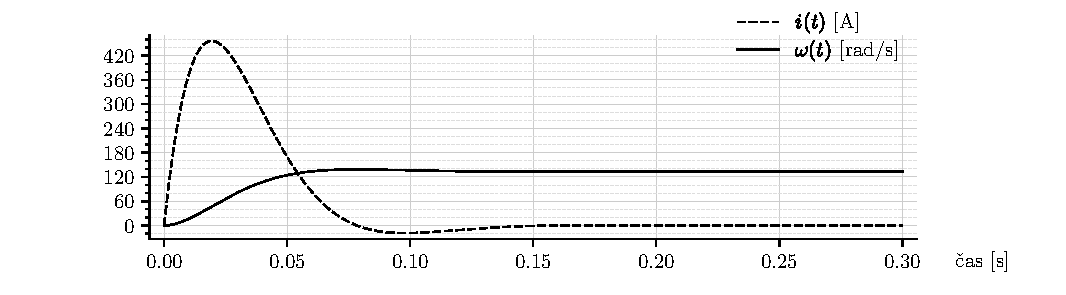
\includegraphics{kMRS02_fig_1.pdf}
		}

	    \figcaption{Grafické znázornenie výsledku numerickej simulácie.}
		\label{Grafické znázornenie výsledku numerickej simulácie}

	\end{center}





\end{enumerate}




\subsection{Vsuvka podľa záujmu}

Opakovanie analytického riešenia diferenciálnych rovníc\ldots





























\section{Cvičenie tretie}


\subsection{Úlohy}

\begin{enumerate}[leftmargin=0pt, labelsep=4mm, itemsep=0pt]

	\item Vytvorte numerickú („počítačovú“) simuláciu časového priebehu výchylky kyvadla (kyvadlo ako nelineárny dynamický systém).

    \begin{itemize}[leftmargin=0pt, labelsep=4mm, itemsep=0pt]
        \item Schematické znázornenie pre implementáciu v prostredí MATLAB-Simulink (základné bloky).
        \item Implementácia s využitím všeobecného ODE solvera.
    \end{itemize}

    \item Simulujte priebeh výchylky kyvadla
    \begin{itemize}[leftmargin=0pt, labelsep=4mm, itemsep=0pt]
        \item[a)] pre začiatočný stav $\varphi = 0,25$ [rad], $\dot\varphi = 0$ [rad/s] a $\ddot\varphi = 0$ [rad/s$^{2}$] pričom $u(t) = 0$ [kg~m$^2$~s$^{-2}$],
        \item[b)] pre skokovú zmenu signálu $u(t)$, ktorá nastane v čase $t=0$ a hodnota signálu sa zmení z \lstyle{0} [kg~m$^2$~s$^{-2}$] na \lstyle{9,81} [kg~m$^2$~s$^{-2}$].
    \end{itemize}

    % \item Porovnajte výstup lineárneho modelu, ako je opísaný v časti~\ref{tdopiscast}, a nelineárneho modelu kyvadla pri vhodne zvolenej simulácii (pripomienka pre cvičiaceho: skoková zmena v okolí pracovného bodu - rôzna veľkosť okolia).


\end{enumerate}





\subsection{Vsuvka podľa záujmu}

\begin{enumerate}[leftmargin=0pt, labelsep=4mm, itemsep=0pt]

    \item Opakovanie analytického riešenia diferenciálnych rovníc\ldots
	
	% \item Porovnajte výstup lineárneho modelu, ako je opísaný v časti~\ref{tdopiscast}, a nelineárneho modelu kyvadla pri vhodne zvolenej simulácii (pripomienka pre cvičiaceho: skoková zmena v okolí pracovného bodu - rôzna veľkosť okolia).
	
\end{enumerate}














\section{Príklady riešených príkladov}



Poznámka: táto časť vznikla v rámci predmetu Projekt -- Odborná prax (Inž. štud. prog. Roborika a kybernetika) v ZS ak. r. 2021/2022 s využitím: \newline {\scriptsize \url{https://math.libretexts.org/Courses/Monroe_Community_College/MTH_225_Differential_Equations}}.



\medskip

\noindent
V tejto časti sa pomocou príkladov venujme riešeniu obyčajných diferenciálnych rovníc s využitím charakteristickej rovnice. Charakteristická rovnica je rovnica $n$-tého stupňa, pomocou ktorej dokážeme získať riešenie diferenciálnych rovníc $n$-tého rádu. Avšak túto metódu výpočtu môžeme použiť len v prípade, že daná diferenciálna rovnica je lineárna.

Pri riešení diferenciálnych rovníc je taktiež potrebné si uvedomiť fakt, že s inými začiatočnými podmienkami sa bude líšiť aj jej riešenie.

Pripomeňme, že pri riešení diferenciálnych pomocou výpočtu koreňov z charakteristickej rovnice môžu nastať 3 prípady, pre ktoré platí

\begin{enumerate}
    \item Ak má charakteristická rovnica $n$ navzájom rôznych riešení $s_{i}$ pre $i = 1, \dots ,n$, potom zodpovedajúce fundamentálne riešenia sú: $e^{s_{1}t}, e^{s_{2}t}, \dots , e^{s_{n}t}$.
    \item Ak sa medzi $n$ koreňmi charakteristického polynómu vyskytne $k$-násobný koreň,
    vytvoríme $k$ lineárne závislých riešení: $e^{s_{i}t}, te^{s_{i}t}, \dots , t^{k-1}e^{s_{i}t}$.
    \item V prípade výskytu dvojice komplexne združených koreňov charakteristického polynómu, $s_{1,2} = \alpha \pm j\beta$, kde $j$ je imaginárna jednotka, využijeme na určenie fundamentálnych riešení Eulerov vzťah
    \begin{equation}
        e^{(\alpha \pm j\beta)t} = e^{\alpha t}(\cos{\beta t} \pm j \sin{\beta t})
    \end{equation}
    
    Potom príslušné fundamentálne riešenie bude v tvare:
    
    \begin{equation}
        c_{1}e^{(\alpha + j\beta)t} + c_{2}e^{(\alpha - j\beta)t} = e^{\alpha t}(c^{'}\cos{\beta t} + c^{'}\sin{\beta t})
    \end{equation}
\end{enumerate}

Ak by sme získali viac fundamentálnych riešení, celkové riešenie diferenciálnej rovnice bude súčet týchto riešení prenásobené $c_{1}, \dots, c_{n}$ reálnymi konštantami, ktoré následne dopočítame zo začiatočných podmienok.





\subsection{Príklad č. 1}

Predpokladajme rozpad rádioaktívneho materiálu, ktorého rýchlosť rozpadu je úmerná hmotnosti prítomného materiálu v čase. Je to obyčajná diferenciálna rovnica prvého rádu v tvare
\begin{equation}\label{eq:rozpad_Q}
    \Dot{Q} = -k \  Q
\end{equation}

pričom $Q$ je hmotnosť rádioaktívneho materiálu v čase $t$ a $k$ je konštanta charakterizujúca rýchlosť rozpadu konkrétneho prvku, ktorú vypočítame ako
\begin{equation}
    k = \frac{\ln{2}}{\tau}
\end{equation}
kde $\tau$ je polčas rozpadu rádioaktívneho materiálu.\\

Aby sme si úlohu skonkretizovali, predpokladajme napríklad izotop $^{228}Ra$ (Rádium), ktorého $\tau = 6.7$ rokov a v čase $t=0$ bude mať hmotnosť $Q_{0} = 4 g$. 


\paragraph{Riešenie}

Rovnicu (\ref{eq:rozpad_Q}) si upravíme tak aby sme všetky neznáme a jej derivácie mali na ľavej strane. 
\begin{equation}\label{eq:rozpad_Q2}
    \Dot{Q} + k \  Q = 0
\end{equation}
Z nej zostavíme charakteristickú rovnicu v tvare
\begin{equation}
    s + k = 0
\end{equation}
Z tejto jednoduchej charakteristickej rovnice vidíme, že obsahuje 1 reálny koreň $s_1 = -k$. Riešenie tejto rovnice teda bude
\begin{equation}
    Q = c_1 e^{-kt}
\end{equation}
kde $c_1$ je reálna konštanta, ktorú vypočítame z predpokladu zadania, že v čase $t = 0$ je $Q(0) = 4$ keďže $Q(0) = c_1 e^{-k 0} = c_1$.
\begin{equation}
    c_{1} = Q_{0} = 4
\end{equation}
Výsledné riešenie našej diferenciálnej rovnice je funkcia
\begin{equation}
    Q = 4 e^{-kt}
\end{equation}







\subsection{Príklad č. 2}

Uvažujme systém s pružinou, na konci ktorej je zavesené závažie s hmotnosťou $m=2$ [kg]. Sily pôsobiace na predmet nech sú: odpor pružiny úmerný k jej predĺženiu (výchylke) $F_1= k y$ a tlmenie pohybu úmerné rýchlosti $F_2 = c v$. Tuhosť pružiny je $k=7$ [N m$^{-1}$] a tlmenie oscilácií $c=0.5$ [N  m$^{-1}$ s]. Začiatočné podmienky systému nech sú: výchylka $y(0) = 1$ [m] a rýchlosť $v(0)=\dot{y}(0) = 1$ [ms$^{-1}$]. Úlohou je nájsť časový priebeh predĺženia (výchylky) pružiny $y$ v čase $t>0$ [s].

\paragraph{Riešenie}

Zostavme diferenciálnu rovnicu podľa druhého Newtonovho pohybového zákona.
\begin{align}
\begin{split}
    F &= - F_1 - F_2 \\
    ma &= -cv - ky 
\end{split}
\end{align}
Úpravou a dosadením konkrétnych koeficientov vznikne diferenciálna rovnica druhého rádu:
\begin{align}
\begin{split}
    m \Ddot{y} + c\Dot{y} + ky &= 0 \\
    2 \Ddot{y} + 0.5\Dot{y} + 7y &= 0
\end{split}
\end{align}
Korene charakteristickej rovnice, ktorá je v tvare
\begin{equation}
    2s^2 + 0.5s + 7 = 0
\end{equation}
sú
\begin{align}
    \begin{split}
        s_{1} &= -0.125 + 1.867i \\
        s_{2} &= -0.125 - 1.867i
    \end{split}
\end{align}


Keďže máme dvojicu komplexne združených koreňov, zapíšeme fundamentálne riešenie v tvare:
\begin{equation}\label{eq:fund_y}
    y_f(t) = c_{1}e^{-0.125}\cos{(1.867t)} + c_{2}e^{-0.125}\sin{(1.867t)}
\end{equation}
Potrebujeme ešte dopočítať koeficienty $c_1$ a $c_2$. Keďže máme 2 neznáme, potrebujeme 2 rovnice aby sme ich vypočítali. Tu znova využijeme hodnoty začiatočných podmienok (stavov), avšak do výrazu (\ref{eq:fund_y}) môžeme dosadiť len začiatočnú polohu. Aby sme vedeli zakomponovať aj začiatočnú rýchlosť, musíme výraz tento výraz zderivovať podľa času (keďže vieme, že rýchlosť je derivácia dráhy podľa času).

\begin{lstlisting}[language=python,float=htpb,label=lst:diff_y,caption={Príklad derivácie výrazu (symbolického) v jazyku Python}]
from sympy import symbols, diff, exp, sin, cos
t, c1, c2 = symbols('t, c1, c2')
y = c1*exp(-0.125*t)*cos(1.867*t) + c2*exp(-0.125*t)*sin(1.867*t)
dy = diff(y, t)
\end{lstlisting}

\begin{align}\label{eq:fund_yy}
    \begin{split}
        \Dot{y_f}(t) = &-1.867c_{1}e^{-0.125t}\sin{(1.867t)} - 0.125c_{1}e^{-0.125t}\cos{(1.867t)} \\
        &- 0.125c_2 e^{-0.125t}\sin{(1.867t)} + 1.867c_2 e^{-0.125t}\cos{(1.867t)}
    \end{split}
\end{align}

Do (\ref{eq:fund_y}) a (\ref{eq:fund_yy}) je možné dosadiť začiatočné podmienky pre čas $t=0$. Získame tak sústavu dvoch rovníc:
\begin{align}
    \begin{split}
        1 &= c_1 \\
        1 &= -0.125c_1 + 1.867 c_2 \hspace{1cm} \Rightarrow \hspace{1cm} c_2 = \frac{1.125}{1.867} = 0.603
    \end{split}
\end{align}
Následne tieto koeficienty dosadíme do (\ref{eq:fund_y}):
\begin{equation}
    y_f(t) = e^{-0.125}\cos{(1.867t)} + 0.603e^{-0.125}\sin{(1.867t)}
\end{equation}







\subsection{Príklad č. 3}

Uvažujme nehomogénnu lineárnu diferenciálnu rovnicu. To znamená, že výstup nebude závisieť len od začiatočných podmienok ale aj od istého vstupného signálu. 

S využitím charakteristickej rovnice hľadajme riešenie úlohy dynamického systému:
\begin{align}
\begin{split}
    \Ddot{y} + 6 \Dot{y} + 10y &= 20t + 22 \\
    y(0) &= 2 \\
    \Dot{y}(0) &= -2
\end{split}
\end{align}
kde $x$ je, samozrejme, odlišné od $y$ a teda rovnica je nehomogénna (neobsahuje len neznámu $y$).


\paragraph{Riešenie}

Konkrétne i v tomto prípade je možné využiť charakteristickú rovnicu.
\begin{equation}
    s^{2} + 6s + 10 = 0  
\end{equation}
Jej riešenie:
\begin{align}
    \begin{split}
        s_1 &= -3 + i \\
        s_2 &= -3 - i 
    \end{split}
\end{align}
Fundamentálne riešenie homogénnej (ľavej strany rovnice) časti teda bude v tvare:
\begin{equation}
    y_{h} = c_1 e^{-3x}\cos{(t)} + c_2 e^{-3x}\sin{(t)}
\end{equation}
Takýto predpis by malo riešenie (funkcia $y(t)$) ak by sa jednalo o homogénny systém. Tu ale musíme brať do úvahy aj nehomogénnu časť. Preto si zavedieme pomocný polynóm predstavujúci tzv. partikulárne riešenie dané nehomogénnou časťou.
\begin{equation}
    y_{p} = At + B \hspace{0.5cm} \Rightarrow \hspace{0.5cm} \Dot{y_{p}} = A \hspace{0.5cm} \Rightarrow \hspace{0.5cm} \Ddot{y_{p}} = 0
\end{equation}
Pre partikulárne riešenie musí platiť (výpočet $A$, $B$) :
\begin{align}
    \begin{split}
        \Ddot{y}_{p} + 6\Dot{y}_{p} + 10 y_{p} &= 6A + 10(At + B) \\
        &=  10At + 6A + 10B  =  20t + 22
    \end{split}
\end{align}
Následne
\begin{equation}
    \begin{pmatrix}
    6 & 10 \\
    10 & 0
    \end{pmatrix}
    \begin{pmatrix}
    A \\
    B
    \end{pmatrix}
    =
    \begin{pmatrix}
    22 \\
    20
    \end{pmatrix}
\end{equation}
Čím sme získali parametre $A=2$ a $B=1$. A teda všeobecné riešenie tohto problému je:
\begin{align}
    \begin{split}
        y_{vs} &= c_1 e^{-3t}\cos{(t)} + c_2 e^{-3t}\sin{(t)} + y_{p} \\
        &= c_1 e^{-3t}\cos{(t)} + c_2 e^{-3t}\sin{(t)} + 2t + 1
    \end{split}
    \end{align}

Následne, koeficienty $c_1$ a $c_2$ dopočítame zohľadnením začiatočných podmienok:
\begin{align}
    \begin{split}
        y(t) &= c_1 e^{-3t}\cos{(t)} + c_2 e^{-3t}\sin{(t)} + 2t + 1 \\
        \Dot{y}(t) &= -c_{1}e^{-3t}\sin{(t)} - 3c_{1}e^{-3t}\cos{(t)} - 3c_{2}e^{-3t}\sin{(t)} + c_{2}e^{-3t}\cos{(t)} + 2 \\
    \end{split}
\end{align}
\begin{align}
    \begin{split}
        y(0) &= 2 = c_{1} \\
        \Dot{y}(0) &= -2 = -3c_{1} + c_{2} + 2 \hspace{0.5cm} \Rightarrow \hspace{0.5cm} c_{2} = 2
    \end{split}
\end{align}
A teda hľadané riešenie bude mať tvar:
\begin{equation}
    y = 2 e^{-3t}\cos{(t)} + 2 e^{-3x}\sin{(t)} + 2t + 1
\end{equation}

























% \pagebreak


\section{Otázky a úlohy}

\begin{enumerate}[leftmargin=0pt, labelsep=3mm, itemsep=0pt]
    
    \item Čo je riešením obyčajnej diferenciálnej rovnice (vo všeobecnosti)?

    \item Vysvetlite rozdiel medzi homogénnou a nehomogénnou obyčajnou diferenciálnou rovnicou.

    \item Uveďte príklad homogénnej obyčajnej diferenciálnej rovnice.

    \item Uveďte príklad nehomogénnej obyčajnej diferenciálnej rovnice.

    \item Vysvetlite pojem \emph{analytické riešenie} obyčajnej diferenciálnej rovnice.

    \item Vysvetlite pojem \emph{numerické riešenie} obyčajnej diferenciálnej rovnice.

    \item Aký je rozdiel medzi analytickým a numerickým riešením diferenciálnej rovnice?

	\item Nájdite analytické riešenie diferenciálnej rovnice (nejaká bude zadaná).
	
    \item Nájdite analytické riešenie diferenciálnej rovnice
    \begin{align*}
        \dot y(t) + a y(t) = 0 \qquad y(0) = y_0 \qquad a\in\mathbb R,\ y_0\in\mathbb R
    \end{align*}

    \item Nájdite analytické riešenie diferenciálnej rovnice
    \begin{align*}
        \ddot y(t) + (a+b) \dot y(t) + ab y(t) = 0 \qquad y(0) = y_0,\ \dot y(0) = z_0  \qquad a\in\mathbb R,\ b\in\mathbb R,\ y_0\in\mathbb R,\ z_0\in\mathbb R
    \end{align*}

    \item Z diferenciálnej rovnice vyššieho rádu zostavte sústavu diferenciálnych rovníc prvého rádu(bude zadaný konkrétny príklad).
    
    \item Nasledujúcu diferenciálnu rovnicu druhého rádu prepíšte na sústavu diferenciálnych rovníc prvého rádu.
    \begin{align*}
        a_2 \ddot y(t) + a_1 \dot y(t) + a_0 y(t) = b_0 u(t) \qquad a_2, a_1, a_0, b_0 \in\mathbb R
    \end{align*}

    \item Sústavu rovníc
    \begin{align*}
        \dot x_1(t) &= x_2(t) \\
        \dot x_2(t) &= - a_0 x_1(t) - a_1 x_2(t) + b_0 u(t) \\
        y(t) &= x_1(t)
    \end{align*}
    prepíšte do maticového tvaru:
    \begin{align*}
        \dot x(t) &= Ax(t) + bu(t) \\
        y(t) &= c^\naT x(t)
    \end{align*}
    (definujte signálny vektor $x(t)$, maticu $A$ a vektory $b$ a $c$).

\end{enumerate}











\end{document}
